\chapter[Consideraciones de diseño]{Consideraciones de diseño\label{cap:consideraciones}}


El proyecto se organiza como un ecosistema modular desacoplado para la instrumentación, recopilación, procesamiento y análisis de manchas solares. Esta organización permite separar responsabilidades entre la adquisición local, la publicación de datos, el procesamiento mediante modelos de Deep Learning y el análisis predictivo de la actividad solar.

\begin{figure}[H]
    \centering
    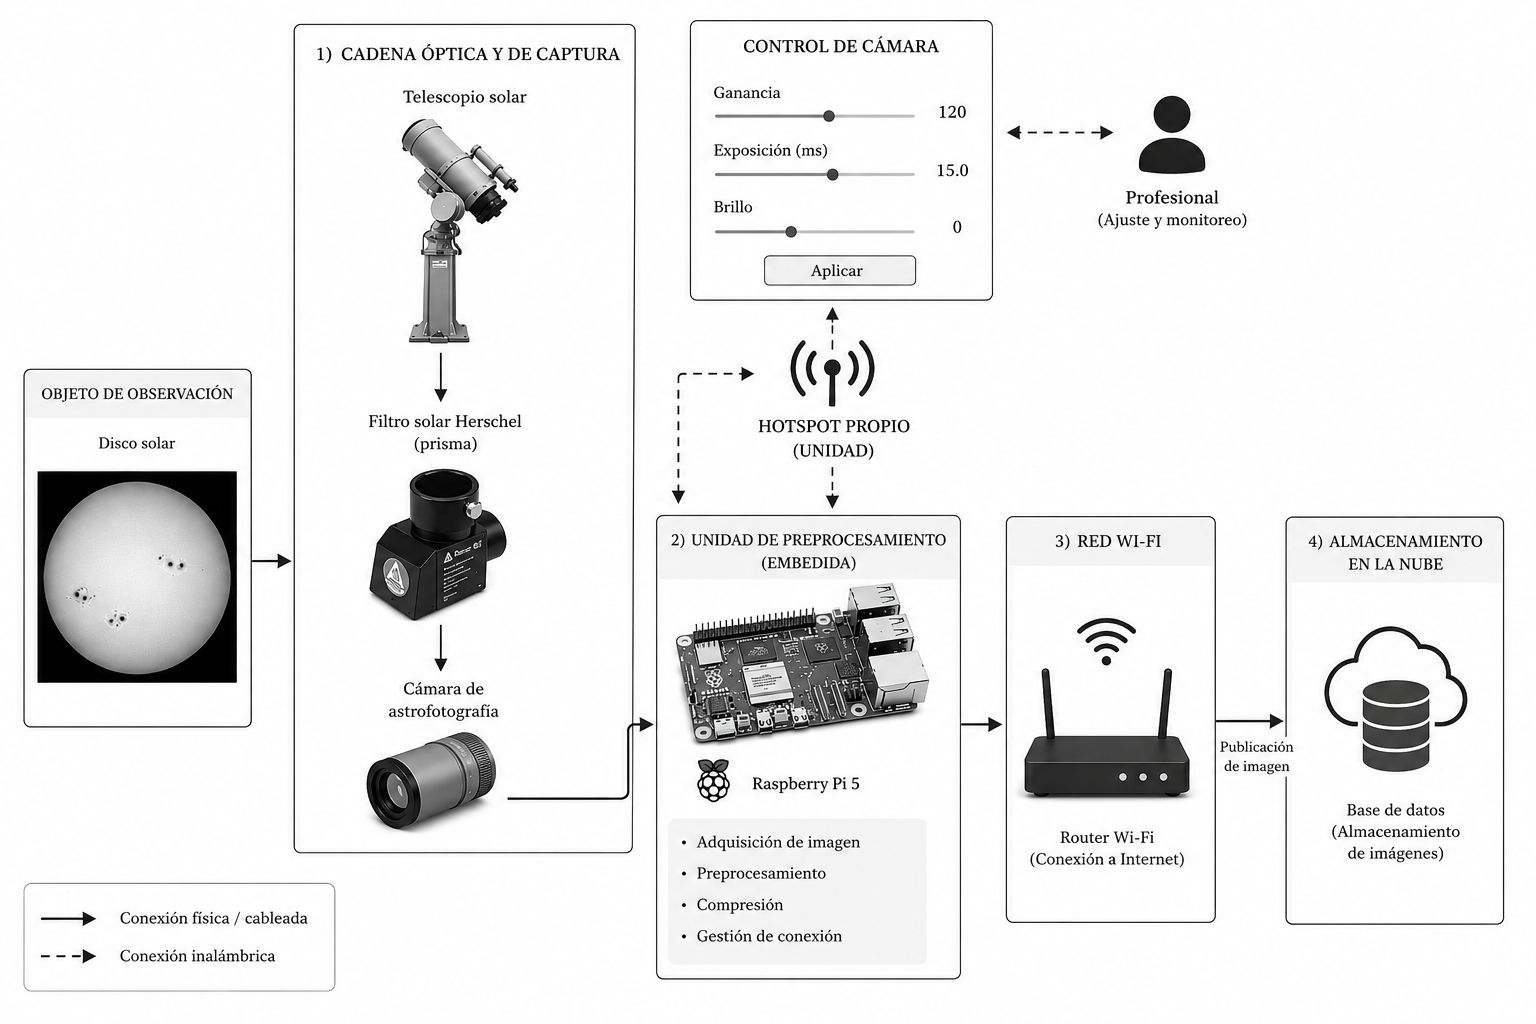
\includegraphics[width=\textwidth]{figures/hw/module.png}
    \caption{Flujo operativo de la etapa de preprocesamiento embebida. Se destaca la captura y calibración de imágenes de disco solar completo, la operación mediante panel web local y la publicación posterior hacia una base de datos en la nube. \textbf{Fuente:} Elaboración propia.}
    \label{fig:ecosistema-modular-general}
\end{figure}

La primera etapa corresponde a la unidad de preprocesamiento embebida. Esta unidad opera junto al sistema óptico de observación y cumple una función dual de conectividad: por un lado, despliega una zona WiFi propia para configuración directa en campo; por otro, puede conectarse como cliente a una red WiFi disponible para la publicación de datos. Desde esta unidad se gestionan la calibración, la captura de imágenes de disco solar completo y las tareas iniciales de preprocesamiento. La operación se controla mediante un panel web en la red local de la propia unidad, lo que permite ajustar parámetros de captura, supervisar el estado del dispositivo y coordinar el envío de observaciones sin depender de una estación externa permanente.

Una vez obtenidas y preprocesadas, las imágenes se envían desde el mismo dispositivo hacia una base de datos en la nube.

\begin{figure}[H]
    \centering
    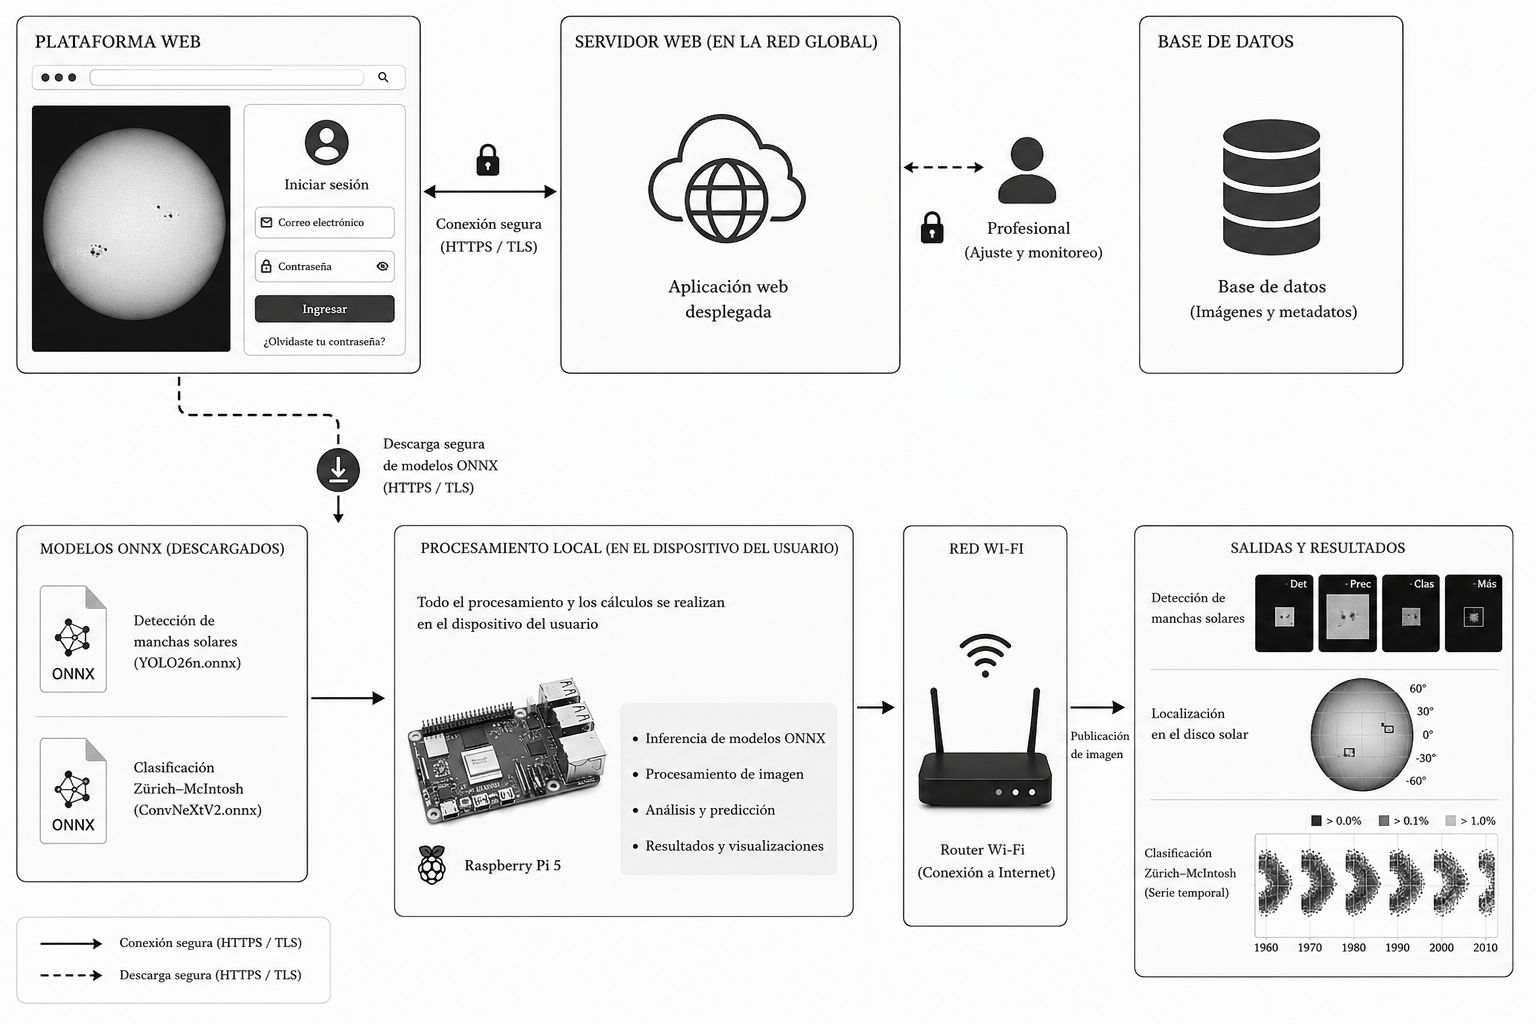
\includegraphics[width=\textwidth]{figures/hw/camera_mount.png}
    \caption{Flujo operativo de la etapa de procesamiento, agrupamiento y clasificación con ONNX y predicción de actividad solar. \textbf{Fuente:} Elaboración propia.}
    \label{fig:unidad-preprocesamiento-embebida}
\end{figure}

Esta base de datos actúa como repositorio intermedio para almacenar imágenes, metadatos y registros observacionales, desacoplando la etapa de adquisición de las etapas posteriores de consulta y análisis.

A partir de estos datos publicados, una segunda plataforma web de acceso abierto recopila y presenta la información disponible. En dicha plataforma se integran los modelos de Deep Learning para el procesamiento de imágenes y la clasificación Zurich--McIntosh, un apartado de tendencias que incorpora los modelos predictivos estudiados, y un apartado de registros destinado a visualizar tanto los datos recopilados para este trabajo como los obtenidos en el Observatorio Astronómico ``Prof. Alexis Troche Boggino''.

\begin{figure}[H]
    \centering
    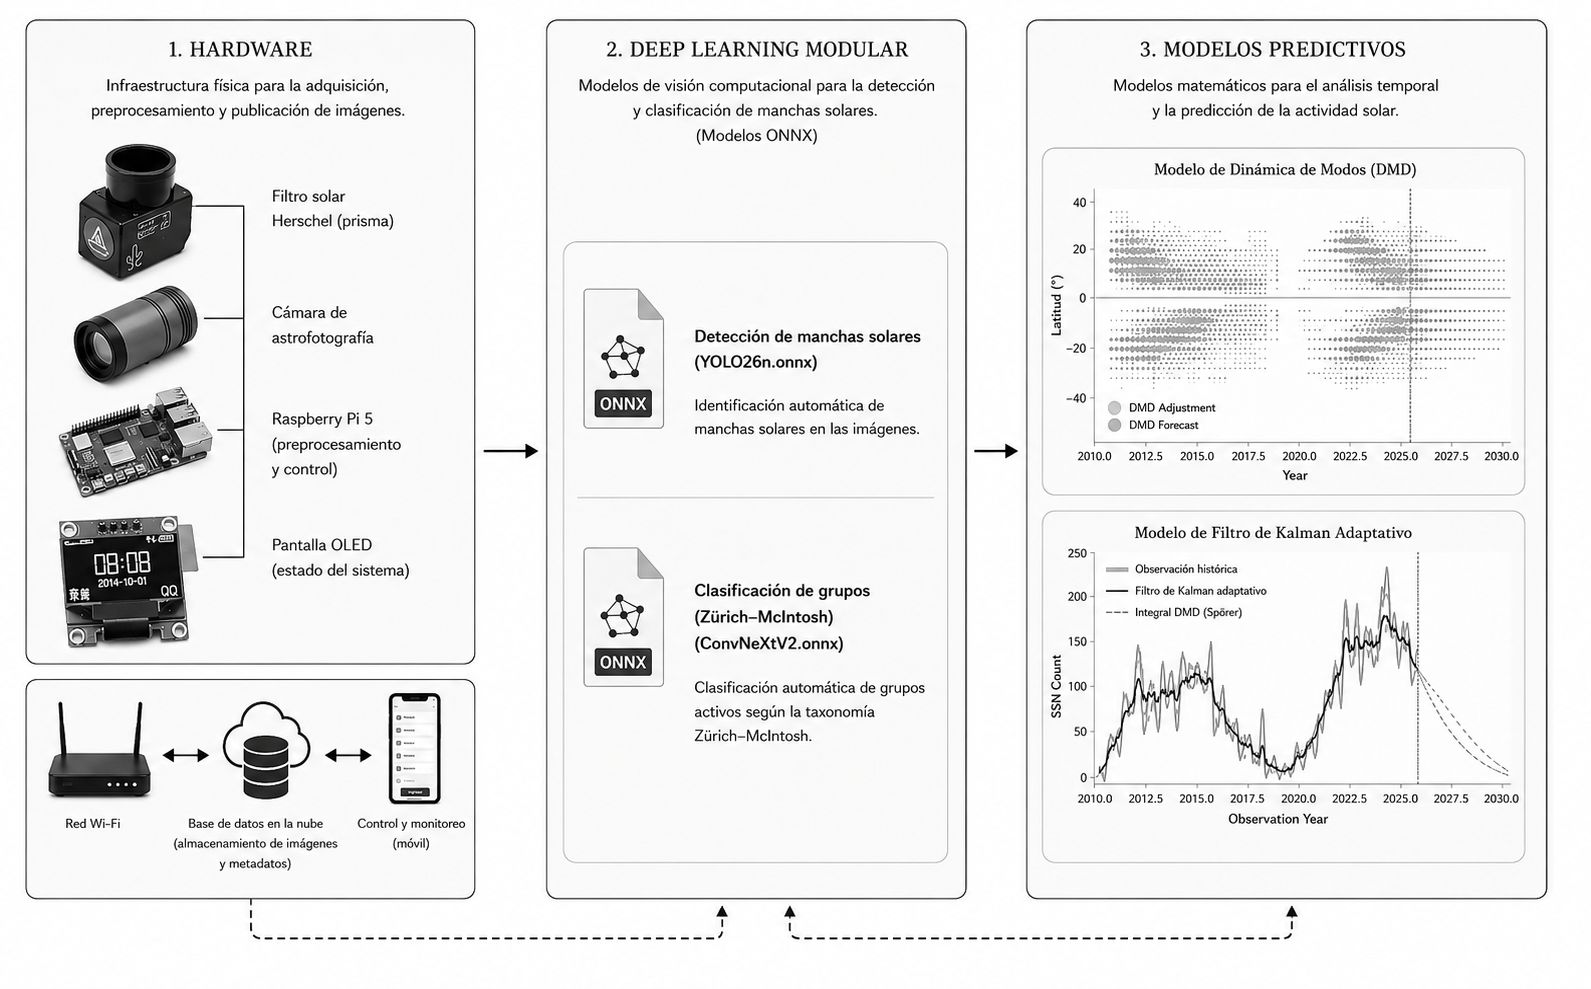
\includegraphics[width=\textwidth]{figures/hw/site_setup.png}
    \caption{Arquitectura integral del ecosistema de trabajo. La figura resume la relación entre la instrumentación solar, la unidad embebida de captura y preprocesamiento, la base de datos en la nube y la plataforma web abierta que integra clasificación Zurich--McIntosh, modelos de tendencias y registros observacionales. \textbf{Fuente:} Elaboración propia.}
    \label{fig:arquitectura-integral-ecosistema}
\end{figure}

La Figura~\ref{fig:arquitectura-integral-ecosistema} resume la relación entre estos elementos. El flujo general parte de la instrumentación solar, continúa con la unidad embebida de captura y preprocesamiento, publica las observaciones en una base de datos en la nube y culmina en una plataforma web abierta donde se concentran los módulos de análisis, visualización y consulta histórica.

En este contexto, las consideraciones de diseño del proyecto se presentan en tres secciones diferenciadas: \textit{hardware} e instrumentación, encargados de la adquisición de imágenes solares; Deep Learning, orientado al procesamiento visual y a la clasificación morfológica; y modelos predictivos, dedicados al análisis de tendencias de la actividad solar. La separación entre módulos permite que cada etapa pueda diseñarse, validarse y actualizarse de manera independiente, manteniendo al mismo tiempo una cadena completa desde la captura del disco solar hasta la interpretación científica de los datos.


\section{Hardware}

Como se indicó en la Sección~\ref{sec:physics}, el componente instrumental del proyecto se contextualiza en el Observatorio Astronómico ``Prof. Alexis Troche Boggino'' y en su infraestructura de supervisión y registro, mostrada en la Figura~\ref{fig:observatorio-alexis-troche}. A partir de ese entorno local, esta sección se concentra en la cadena de hardware específica del prototipo.

Para el prototipo se considera una cadena de instrumentación para luz blanca compuesta por un telescopio refractor Vixen con diámetro $D=60\,\mathrm{mm}$ y distancia focal $F=420\,\mathrm{mm}$, una cámara monocromática y un filtro de atenuación óptica adecuado para observación solar. Este conjunto establece las condiciones de exposición, contraste, campo de visión y estabilidad mecánica sobre las que luego operan las etapas de preprocesamiento y análisis. El uso de un refractor pequeño favorece la portabilidad, reduce exigencias mecánicas, facilita la alineación en pruebas de campo y permite implementar medidas de seguridad óptica con menor complejidad que en instrumentos de mayor apertura. Posteriormente, se selecciona la plataforma base para el desarrollo del módulo de adquisición de imagen y preprocesamiento embebido.

\subsection{Cámara de astrofotografía solar}

La selección de la cámara se abordó como una exploración del mercado de sensores monocromáticos empleados en imagen solar de alta cadencia. Dado que la cámara seleccionada debe integrarse en un tren óptico compacto y ofrecer una base útil para captura solar rápida, la comparación se centra en prestaciones directamente vinculadas con ese objetivo: área sensora, resolución espacial, tamaño de píxel, tipo de obturador, conversión ADC, interfaz y precio referencial. La Tabla~\ref{tab:comparacion_camaras_proyecto} resume estas variables para un conjunto de alternativas monocromáticas disponibles comercialmente \citep{zwoASI174Manual2025,zwoGuideCameras2025,qhyQHY5III6782026,qhyMiniCAM8M2026,playerOneApolloMMax2026}.

\begin{table}[H]
\centering
\caption{Exploración de cámaras monocromáticas disponibles comercialmente para captura solar de alta cadencia y guiado. Los precios son referenciales y pueden variar según distribuidor, región y fecha de consulta. \textbf{Fuente:} Elaboración propia.}
\label{tab:comparacion_camaras_proyecto}
\uniformtablestyle
\begin{tabularx}{\textwidth}{>{\raggedright\arraybackslash}p{2.9cm} >{\raggedright\arraybackslash}p{2.8cm} >{\raggedright\arraybackslash}p{2.15cm} >{\centering\arraybackslash}p{1.3cm} X}
\toprule
\textbf{Fabricante / modelo} & \textbf{Sensor / muestreo} & \textbf{Conversión / interfaz} & \textbf{Precio ref.} & \textbf{Observaciones} \\
\midrule
QHYCCD QHY5III678M & IMX678, 7.71\,mm $\times$ 4.36\,mm; 3856$\times$2180; 2.0\,$\mu$m & 12-bit ADC; USB3.0 Tipo-C; buffer 512 MB & US\$384 & Destaca por su resolución de 8.4 MP y por un muestreo fino basado en píxeles de 2.0\,$\mu$m. \\
ZWO ASI174MM Mini & IMX174LLJ/LQJ, 11.3\,mm $\times$ 7.1\,mm; 1936$\times$1216; 5.86\,$\mu$m & 12-bit ADC; QE pico 77\%; USB2.0 Tipo-C & US\$432 & Destaca por combinar sensor de 1/1.2\,$''$, obturador global y píxeles de 5.86\,$\mu$m en formato mini. \\
QHYCCD miniCAM8M & IMX585, 11.2\,mm $\times$ 6.3\,mm; 3856$\times$2180; 2.9\,$\mu$m & Dual 12-bit ADC; USB3.0; TEC; carrusel 8 pos. & US\$599 & Destaca por integrar refrigeración TEC y carrusel de filtros en un cuerpo orientado a captura más versátil. \\
Player One Apollo-M MAX & IMX432, 14.5\,mm $\times$ 9.9\,mm; 1608$\times$1104; 9.0\,$\mu$m & 12-bit ADC; USB3.0; obturador global & US\$618 & Destaca por su área sensora amplia y por píxeles de 9.0\,$\mu$m orientados a alta señal por píxel. \\
\bottomrule
\end{tabularx}
\end{table}

A partir de esta comparación se adopta la ZWO ASI174MM Mini como dispositivo principal de captura. Su rasgo diferencial dentro del conjunto evaluado es la combinación entre sensor de 1/1.2\,$''$, obturador global, píxel de 5.86\,$\mu$m y cuerpo mini, una combinación poco frecuente cuando se busca compatibilidad con trenes ópticos compactos sin comprometer el campo útil ni la robustez temporal en secuencias rápidas \citep{zwoASI174Manual2025,zwoGuideCameras2025,qhyQHY5III6782026,qhyMiniCAM8M2026,playerOneApolloMMax2026}.

\begin{figure}[H]
    \centering
    \begin{subfigure}[t]{0.47\textwidth}
        \centering
        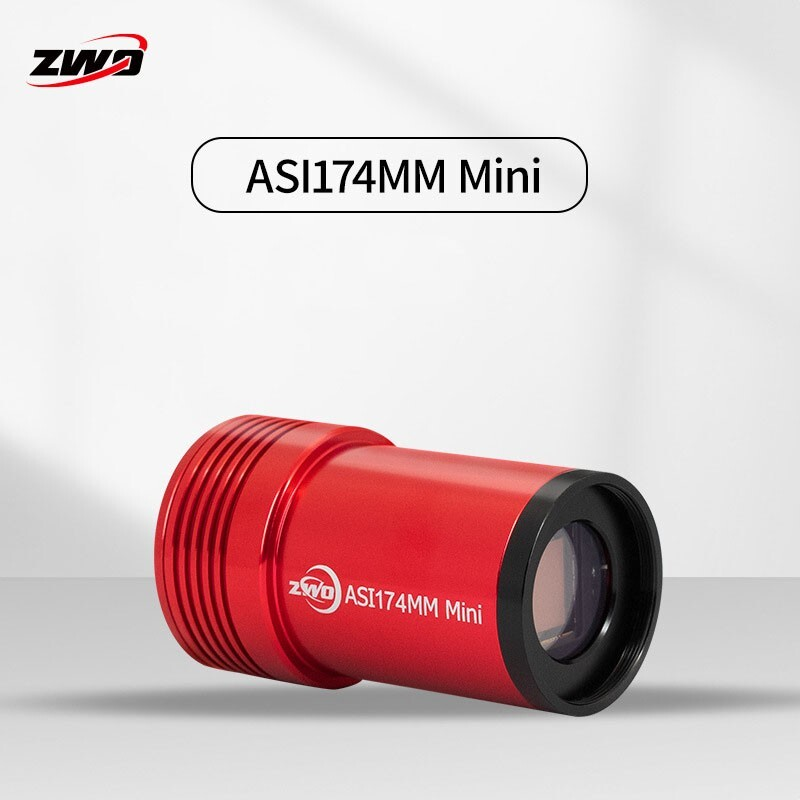
\includegraphics[width=\textwidth]{figures/hw/pi5.jpg}
        \caption{Vista general de la cámara ZWO ASI174MM Mini empleada como dispositivo de captura en el prototipo.}
    \end{subfigure}
    \hfill
    \begin{subfigure}[t]{0.47\textwidth}
        \centering
        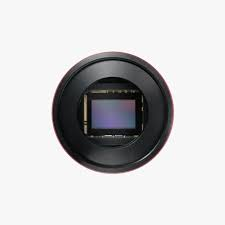
\includegraphics[width=\textwidth]{figures/hw/asi174.jpg}
        \caption{Vista frontal del sensor, donde se aprecia el área sensible del detector CMOS monocromático.}
    \end{subfigure}
    \caption{Cámara ZWO ASI174MM Mini considerada para el prototipo de observación solar. Se muestran (a) la vista general del cuerpo de cámara y (b) la vista frontal del sensor. \textbf{Fuente:} página oficial de ZWO (ZWO Astronomy Cameras).}
    \label{fig:zwo_project_camera}
\end{figure}

La documentación técnica de ZWO reporta para este modelo un área efectiva de 11.3\,mm $\times$ 7.1\,mm, conversión ADC de 12 bits y un QE pico de 77\%. Dentro de la serie mini, además, el fabricante la presenta como la opción de mayor campo y como una cámara pensada para integrarse mecánicamente de forma semejante a un ocular, rasgo relevante para el montaje previsto en este trabajo \citep{zwoASI174Manual2025,zwoGuideCameras2025}.

Desde una perspectiva observacional, el uso de \textit{global shutter} que integra esta cámara contribuye a reducir distorsiones temporales entre líneas y favorece la captura de secuencias rápidas en presencia de \textit{seeing} variable. Asimismo, el carácter monocromático del sensor evita la interpolación cromática asociada a matrices Bayer y conserva mejor la nitidez espacial efectiva. En conjunto, estas propiedades hacen que la cámara resulte particularmente adecuada para registrar estructuras fotosféricas con un balance favorable entre señal por píxel, estabilidad temporal y simplicidad de integración \citep{sonyPregiusGlobalShutter,zwoASI174Manual2025}.

Desde el punto de vista operativo, la combinación entre exposición, ganancia y frecuencia de cuadro debe ajustarse según el brillo fotosférico, la apertura efectiva del sistema y las condiciones atmosféricas. En observación solar, el objetivo no es solo evitar saturación, sino también conservar contraste en umbra y penumbra, sostener una cadencia útil para mitigar el \textit{seeing} y mantener una señal adecuada para el procesamiento posterior. En ese sentido, la cámara se selecciona no únicamente por sus especificaciones nominales, sino por su compatibilidad con el flujo previsto de adquisición local e inferencia posterior.

\begin{figure}[H]
    \centering
    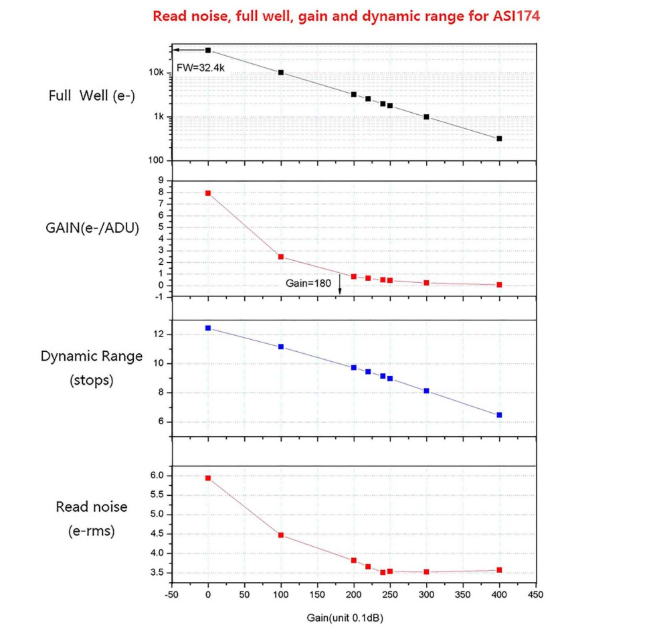
\includegraphics[width=0.78\textwidth]{figures/hw/cam_specs.png}
    \caption{Curvas de pozo completo, ganancia, rango dinámico y ruido de lectura reportadas para la cámara ASI174 en función de la ganancia de adquisición. \textbf{Fuente:} página oficial de ZWO (ZWO Astronomy Cameras).}
    \label{fig:camara-metricas-asi174}
\end{figure}

La Figura~\ref{fig:camara-metricas-asi174} complementa la selección de la cámara al mostrar cómo varían sus parámetros de operación con la ganancia. A ganancia baja, el sensor conserva una mayor capacidad de pozo completo, cercana a $32.4\,\mathrm{ke^-}$, y un rango dinámico superior a 12 pasos, condición favorable cuando se busca evitar saturación en regiones fotosféricas brillantes. Al incrementar la ganancia, la conversión en $\mathrm{e^-}/\mathrm{ADU}$ disminuye y el ruido de lectura se reduce hasta valores próximos a $3.5$--$4\,\mathrm{e^-_{rms}}$, pero también cae el pozo completo y el rango dinámico. Por ello, en el prototipo la ganancia debe elegirse como un compromiso: valores moderados permiten mejorar la sensibilidad aparente y la cadencia práctica, mientras que ganancias excesivas pueden limitar la capacidad de registrar simultáneamente detalles débiles y zonas brillantes sin saturación.

\subsection{Filtro solar y atenuación óptica}

En observación solar de luz blanca, la cuña de Herschel constituye una de las soluciones más eficaces para obtener una atenuación segura y una imagen de alto contraste en telescopios refractores, ya que desvía la mayor parte de la energía incidente fuera del eje óptico útil y deja pasar solo una fracción controlada hacia el sensor. Dado que la cámara seleccionada se integra en un tren óptico de 1.25\,$''$, la exploración del bloque de atenuación se restringe a cuñas de Herschel compatibles con ese diámetro. Bajo esta restricción, dejan de ser relevantes opciones de 2\,$''$ o filtros frontales de apertura completa, y el análisis se concentra en accesorios de 1.25\,$''$ que puedan acoplarse sin introducir adaptaciones innecesarias. Para mantener un criterio técnico comparable, la Tabla~\ref{tab:comparacion_filtros_proyecto} reúne características fundamentales de mercado: diámetro mecánico, presencia de filtrado integrado, compatibilidad con refractores y rasgos constructivos de interés para captura solar. El objetivo es contrastar cuñas de Herschel integrables dentro del mismo tren óptico de la cámara \citep{zwoASI174Manual2025,luntWhiteLightWedges2026,altairHerschelWedge2026,baaderHerschelUsage2026,apmLuntContinuum2026}.

\begin{table}[H]
\centering
\caption{Exploración de accesorios de atenuación solar compatibles con tren óptico de 1.25\,$''$. Los precios son referenciales y se expresan en dólares estadounidenses. \textbf{Fuente:} Elaboración propia.}
\label{tab:comparacion_filtros_proyecto}
\uniformtablestyle
\begin{tabularx}{\textwidth}{>{\raggedright\arraybackslash}p{3.35cm} >{\raggedright\arraybackslash}p{3.15cm} >{\centering\arraybackslash}p{1.45cm} X}
\toprule
\textbf{Fabricante / modelo} & \textbf{Característica técnica} & \textbf{Precio ref.} & \textbf{Observaciones} \\
\midrule
Altair Astro Solar Herschel Wedge 1.25\,$''$ & Variante de 1.25\,$''$ para refractores; orientada a imagen solar & US\$171 aprox. & Se destaca por su formato diagonal compacto y por una superficie cerámica pensada para disipación térmica. \\
Omegon Herschel Prism Tess 1.25\,$''$ & Filtro ND integrado; polarizador incorporado; rosca T2; compatibilidad 1.25\,$''$ & US\$229 & Se destaca por integrar conexión T2 para cámara y control de transmisión incorporado en la propia cuña. \\
Lunt Solar Systems White Light Solar Wedge 1.25\,$''$ & Filtro ND3 preinstalado; carcasa cerrada; trampa de luz integrada; uso en refractores hasta 4\,$''$ & US\$308 & Se destaca por ofrecer un sistema cerrado con trampa de luz interna y configuración lista para observación e imagen solar. \\
APM / Lunt Solar Wedge 1.25\,$''$ + Solar Continuum & ND3 preinstalado; filtro Solar Continuum incluido; uso en refractores & US\$345 aprox. & Se destaca por añadir un filtrado de contraste específico para realce fotosférico sobre la misma base óptica de Lunt. \\
\bottomrule
\end{tabularx}
\end{table}

Sobre esta base, el prototipo adopta la Lunt Solar Systems White Light Solar Wedge de 1.25\,$''$ como elemento principal de atenuación solar. La elección se apoya en un conjunto de rasgos funcionales que la distinguen dentro del grupo evaluado: filtro ND3 preinstalado, carcasa completamente cerrada, trampa de luz integrada y una orientación explícita del fabricante hacia observación e imagen solar en refractores. Estos elementos reducen luz parásita, simplifican la cadena óptica y dejan la cuña lista para uso seguro sin depender de accesorios adicionales para la atenuación primaria. Frente a opciones más económicas, Lunt ofrece una implementación más cerrada y directamente orientada a seguridad operacional; frente a configuraciones más costosas, como el paquete APM/Lunt con Solar Continuum, conserva la misma base óptica con menor complejidad y costo inicial \citep{luntWhiteLightWedges2026,altairHerschelWedge2026,apmLuntContinuum2026}.

\begin{figure}[H]
    \centering
    \begin{subfigure}[t]{0.47\textwidth}
        \centering
        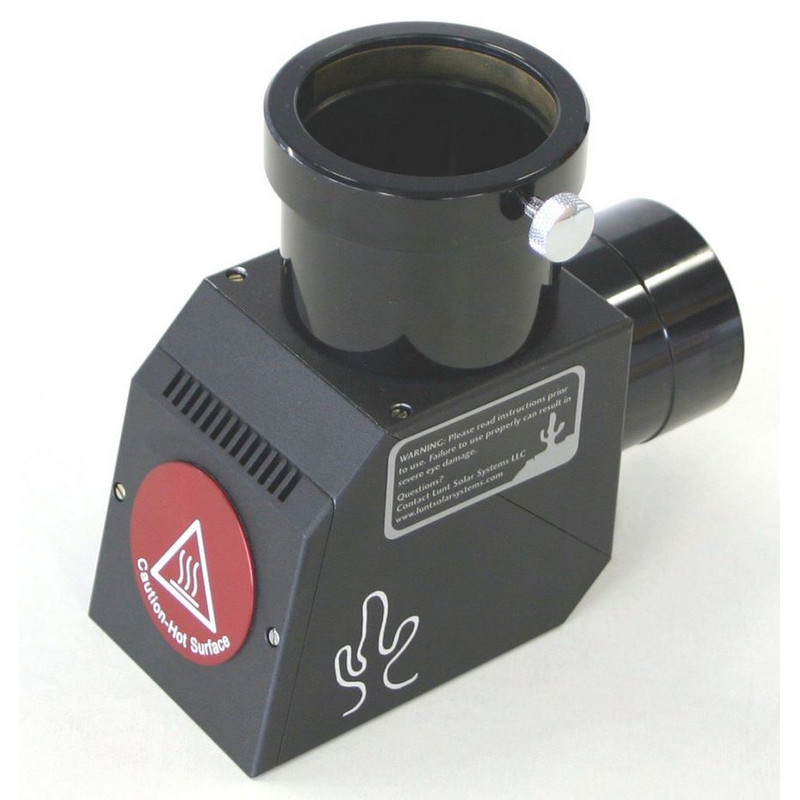
\includegraphics[width=\textwidth]{figures/hw/wedge.png}
        \caption{Prisma Herschel Lunt Solar Systems White Light Solar Wedge de 1.25\,$''$.}
    \end{subfigure}
    \hfill
    \begin{subfigure}[t]{0.40\textwidth}
        \centering
        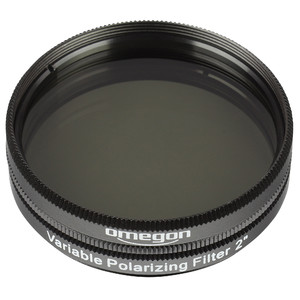
\includegraphics[width=\textwidth]{figures/hw/filter.png}
        \caption{Filtro ND3 interior del prisma.}
    \end{subfigure}
    \caption{Bloque de atenuación solar adoptado para el prototipo. Se muestran (a) el prisma Herschel Lunt de 1.25\,$''$ y (b) el filtro ND3 asociado al conjunto. \textbf{Fuente:} página oficial de Lunt Solar Systems.}
    \label{fig:herschel_project_filter}
\end{figure}

La documentación técnica insiste tanto en la presencia del filtro ND3 o del control de brillo asociado como en la prohibición de colocar filtros por delante de la cuña, precisamente por la carga térmica concentrada en ese punto del sistema \citep{luntWhiteLightWedges2026,altairHerschelWedge2026,baaderHerschelUsage2026}.

Como accesorio complementario, un polarizador puede emplearse después de la cuña para realizar un ajuste fino del brillo durante observación visual o captura. No obstante, su función es secundaria respecto del prisma de Herschel: la atenuación primaria y la seguridad óptica del sistema recaen en la cuña, mientras que la polarización solo modula la transmisión final según las condiciones de trabajo \citep{luntPolarizerWedge2026,baaderSinglePolarizer2026,baaderHerschelUsage2026}. 


\subsection{Plataforma de preprocesamiento y adquisición embebida}

Una vez definido el bloque instrumental, el siguiente componente es la plataforma
embebida encargada de coordinar la captura, ejecutar el preprocesamiento inicial,
almacenar temporalmente las observaciones y despachar la inferencia local. En
este trabajo, esta plataforma debe entenderse como la placa controladora de la
estación de observación, ya que concentra tanto la interacción con la cámara como
la lógica operativa del nodo en campo.

Desde el punto de vista funcional, la placa seleccionada debe reunir al menos
cuatro características. Primero, debe ofrecer capacidad suficiente de
procesamiento de imagen para controlar la cámara, ejecutar tareas de recorte,
normalización, compresión y validación básica de calidad, además de admitir
modelos ligeros de inferencia local. Segundo, debe soportar conectividad dual,
permitiendo operar tanto como cliente WiFi hacia una red disponible como en modo
\textit{hotspot} para configuración y monitoreo local cercano. Tercero, debe
mantener compatibilidad con distribuciones Linux estables, de preferencia Ubuntu
o Debian, para simplificar despliegue, mantenimiento y automatización. Cuarto,
debe ofrecer una ruta de integración práctica con el SDK de ZWO en entorno ARM,
de modo que la adquisición no dependa de software interactivo, sino de bibliotecas
programables \citep{nmcliHotspot2026,zwoASILinuxManual}.

Bajo estos criterios, la Tabla~\ref{tab:comparacion_plataformas_embebidas}
resume algunas opciones de mercado plausibles para una estación compacta de
adquisición solar \citep{raspberryPi5Docs2026,jetsonOrinNanoGuide2026,orangePi5Plus2026,rock5bDocs2026}.

\begin{table}[H]
\centering
\caption{Comparación de plataformas evaluadas para adquisición y preprocesamiento embebido en el prototipo. Los precios son referenciales y pueden variar según configuración, distribuidor y fecha de consulta. \textbf{Fuente:} Elaboración propia.}
\label{tab:comparacion_plataformas_embebidas}
\uniformtablestyle
\begin{tabularx}{\textwidth}{>{\raggedright\arraybackslash}p{2.65cm} >{\raggedright\arraybackslash}p{2.75cm} X >{\centering\arraybackslash}p{1.35cm} >{\raggedright\arraybackslash}p{2.55cm}}
\toprule
\textbf{Placa} & \textbf{Procesamiento de imagen} & \textbf{Características} & \textbf{Precio ref.} & \textbf{Observaciones} \\
\midrule
Raspberry Pi 5 (8 GB) & Broadcom BCM2712; CPU Cortex-A76 4 núcleos a 2.4 GHz; 8 GB LPDDR4X. & WiFi integrado doble banda; modo cliente/AP viable; alimentación 5 V, hasta 5 A. & US\$190 & Mejor equilibrio para estación portátil replicable. \\

NVIDIA Jetson Orin Nano & Arm Cortex-A78AE 6 núcleos; GPU Ampere 1024 CUDA; hasta 40 TOPS; 8 GB LPDDR5. & WiFi no integrado en módulo base; modo dual depende de adaptador; alimentación 19 V, aprox. 2.4 A en kit. & US\$249 & Mayor potencia, más costo y complejidad. \\

Orange Pi 5 Plus & RK3588; CPU 8 núcleos hasta 2.4 GHz; NPU 6 TOPS; 8--16 GB LPDDR4X. & WiFi no integrado; requiere módulo; modo dual depende del adaptador; alimentación 5 V, 4 A. & US\$149 & Buen rendimiento, integración menos directa. \\

ROCK 5B & RK3588; CPU 8 núcleos hasta 2.4 GHz; NPU 6 TOPS; 8--16 GB LPDDR4X. & WiFi no integrado; expansión M.2/E-key; modo dual depende del módulo; alimentación 5 V, hasta 5 A. & US\$145 & Potente, pero menos replicable. \\
\bottomrule
\end{tabularx}
\end{table}

A partir de esta comparación, se adopta la Raspberry Pi 5 en su variante de
8\,GB de RAM como placa controladora del sistema. La decisión no se fundamenta
únicamente en su capacidad de cómputo, suficiente para adquisición,
preprocesamiento e inferencia preliminar, sino también en su integración
inalámbrica nativa. Entre las alternativas evaluadas, es la opción que incorpora
WiFi de doble banda en la propia placa y permite una configuración práctica de
operación dual: punto de acceso local para control en campo y cliente de red para
sincronización de datos. Esta característica reduce adaptadores externos,
simplifica el montaje y mejora la portabilidad del prototipo. Además, la
disponibilidad de distribuciones Linux maduras y la integración efectiva con el
SDK de ZWO en entorno ARM reducen el riesgo de implementación y favorecen la
replicabilidad experimental \citep{raspberryPi5Docs2026,nmcliHotspot2026,zwoASILinuxManual}.


\begin{figure}[H]
    \centering
    \begin{subfigure}[t]{0.47\textwidth}
        \centering
        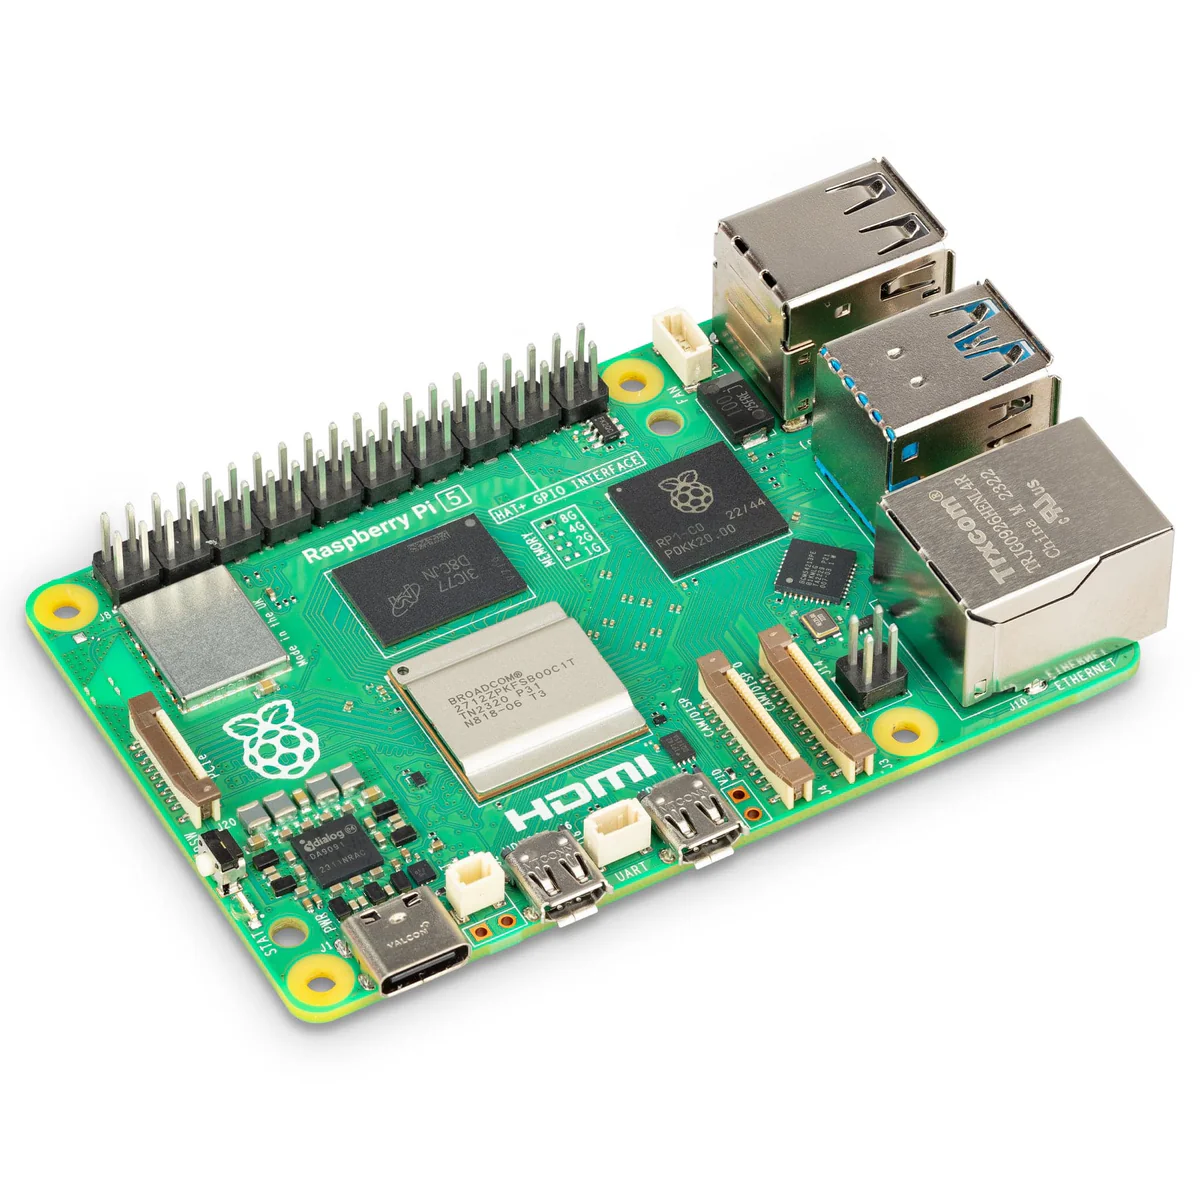
\includegraphics[width=\textwidth]{figures/hw/proc_unit.png}
        \caption{Imagen actual de la plataforma basada en Raspberry Pi 5.}
    \end{subfigure}
    \hfill
    \begin{subfigure}[t]{0.47\textwidth}
        \centering
        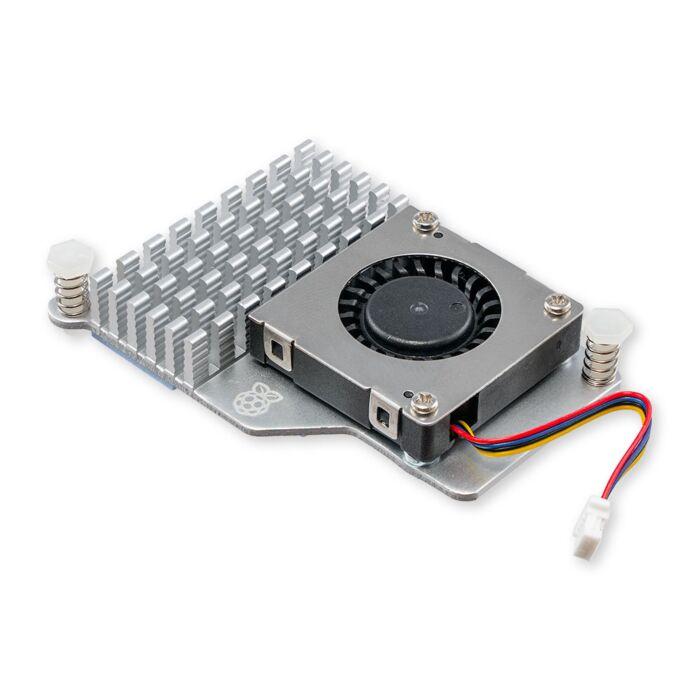
\includegraphics[width=\textwidth]{figures/hw/pi_cooler.jpg}
        \caption{\textit{Cooler} de disipación empleado sobre el procesador.}
    \end{subfigure}
    \caption{Plataforma embebida basada en Raspberry Pi 5 utilizada en el prototipo. Se muestran (a) la integración actual de la placa y (b) el sistema de disipación activa empleado para sostener operación continua en tareas de adquisición y preprocesamiento. \textbf{Fuente:} página oficial de Raspberry Pi.}
    \label{fig:rpi5_embebida_proyecto}
\end{figure}

A su vez, se emplea un
\textit{cooler} sobre el procesador para reducir el sobrecalentamiento y limitar
episodios de \textit{thermal throttling} durante sesiones prolongadas de
adquisición, preprocesamiento e inferencia. Esto resulta pertinente porque la
observación solar puede requerir secuencias continuas, transferencia de imágenes
y ejecución repetida de modelos, cargas que elevan la temperatura del chip.

\section{Procesamiento de imagen}

El procesamiento de imagen se organiza como una cadena modular que transforma
una imagen de disco solar completo en una recomendación taxonómica
Zurich--McIntosh. La Sección~\ref{sec:arquitectura-dl-cascada} describe el flujo
general de modelos y transformaciones entre etapas, mientras que la
Sección~\ref{sec:classification} formaliza la normalización bayesiana utilizada
para obtener la distribución final de recomendación.

\subsection{Arquitectura modular de Deep Learning en cascada}
\label{sec:arquitectura-dl-cascada}

\begin{figure}[H]
    \centering
    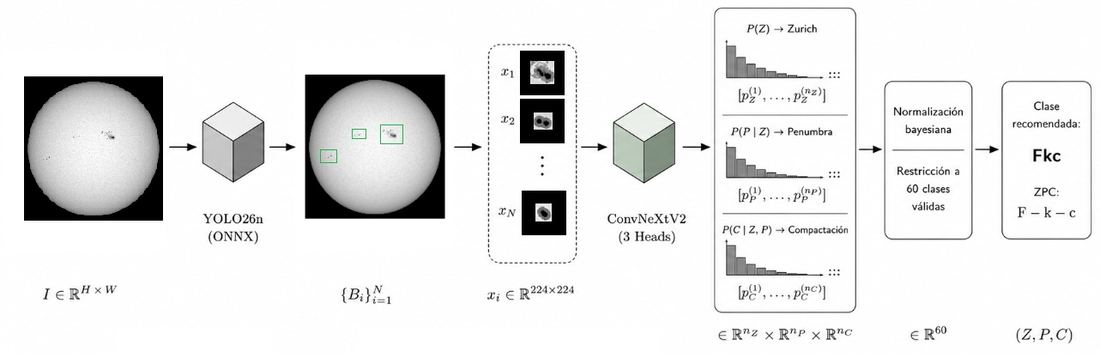
\includegraphics[width=1\textwidth]{figures/sys/img_pipe.jpg}
    \caption{Arquitectura modular en cascada para el procesamiento de imágenes solares. \textbf{Fuente:} Elaboración propia.}
    \label{fig:arquitectura-cascada-imagen}
\end{figure}

La Figura~\ref{fig:arquitectura-cascada-imagen} presenta la arquitectura de
procesamiento como una cascada de modelos y transformaciones intermedias. La primera etapa corresponde a la normalización geométrica de la imagen de disco
solar completo. En este nodo se centra el disco, se recorta la región útil y se
reescalan los datos a $640\times640$ píxeles. Esta salida constituye la entrada
del detector y reduce variaciones de escala y encuadre entre observaciones.

La segunda etapa corresponde a la detección con YOLO26n. El modelo identifica
regiones candidatas mediante \textit{bounding boxes}; cada caja representa un
grupo solar localizado sobre el disco. Esta etapa no asigna la clase
Zurich--McIntosh, sino que delimita las zonas que serán evaluadas por el
clasificador.

La tercera etapa transforma cada caja detectada en un recorte normalizado. Para
ello, la región delimitada se extrae de la imagen y se inserta en un lienzo de
$224\times224$ píxeles, preservando la relación de aspecto para evitar
distorsiones geométricas. El resultado es una colección de imágenes locales
homogéneas para la etapa de clasificación.

La cuarta etapa utiliza un clasificador jerárquico basado en ConvNeXtV2 Atto. Para
cada recorte, el backbone extrae una representación compacta y etapas MLP
complementarias inyectan la dependencia jerárquica entre los caracteres $Z$, $P$
y $C$ de la taxonomía Zurich--McIntosh. Estas salidas no constituyen todavía una
recomendación única, sino una representación probabilística separada por
componente, diseñada además para una conversión íntegra hacia ONNX.

La etapa final aplica normalización bayesiana sobre las salidas del
clasificador. En este bloque se combinan las probabilidades de $Z$, $P$ y $C$, se
anulan combinaciones taxonómicamente inválidas y se renormaliza la distribución
sobre las 60 clases admisibles. La clase con mayor probabilidad en este vector
final se toma como recomendación del sistema.

\subsection{Posprocesamiento con Normalización Bayesiana}

\label{sec:classification}

La dependencia semántica entre componentes se incorpora explícitamente mediante una formulación probabilística jerárquica que respeta la estructura observacional del esquema McIntosh. Para una imagen de entrada $x$, el objetivo es estimar la probabilidad conjunta de la tripleta $(Z,P,C)$, donde $Z$ representa el tipo de grupo, $P$ el carácter penumbral y $C$ la distribución interna del grupo. En su forma base, esta descomposición puede escribirse como
\begin{equation}
P(Z,P,C\mid x)=P(Z\mid x)\,P(P\mid Z,x)\,P(C\mid Z,P,x),
\end{equation}
lo que preserva la naturaleza jerárquica de la clasificación Zurich--McIntosh \citep{mcintosh1990classification}.

En la práctica, sin embargo, el modelo implementado produce tres salidas marginales para $Z$, $P$ y $C$ sin modelar de forma explícita todas las dependencias condicionales. Bajo esta aproximación operativa, se adopta
\begin{equation}
P(P\mid Z,x)\approx P(P\mid x),
\qquad
P(C\mid Z,P,x)\approx P(C\mid x),
\end{equation}
y por tanto se define una probabilidad base factorizada como
\begin{equation}
P_{\mathrm{base}}(Z,P,C\mid x)=P(Z\mid x)\,P(P\mid x)\,P(C\mid x).
\end{equation}
Esta construcción conserva la interpretabilidad del modelo multisalida y permite combinar las tres salidas dentro de una misma regla probabilística de recomendación.

Para imponer consistencia taxonómica se introduce una máscara binaria $M_{ZPC}\in\{0,1\}$, donde $M_{ZPC}=1$ si la combinación es válida dentro del esquema McIntosh y $M_{ZPC}=0$ en caso contrario. Con esta restricción se define la distribución truncada
\begin{equation}
\widetilde{P}(Z,P,C\mid x)=P_{\mathrm{base}}(Z,P,C\mid x)\,M_{ZPC},
\end{equation}
que anula combinaciones físicamente o taxonómicamente incompatibles. Para recuperar una distribución probabilística válida sobre el subconjunto de tripletas aceptadas, se aplica una renormalización bayesiana de la forma
\begin{equation}
P_{\mathrm{rec}}(Z,P,C\mid x)=
\frac{\widetilde{P}(Z,P,C\mid x)}{\sum_{z,p,c}\widetilde{P}(z,p,c\mid x)}
=
\frac{P_{\mathrm{base}}(Z,P,C\mid x)\,M_{ZPC}}{\sum_{z,p,c}P_{\mathrm{base}}(z,p,c\mid x)\,M_{zpc}},
\end{equation}
de modo que la masa total de probabilidad queda normalizada a uno sobre las combinaciones válidas. Esta reformulación permite interpretar $P_{\mathrm{rec}}$ como una distribución coherente para recomendación, ranking y análisis posterior.

La clase recomendada se obtiene entonces mediante
\begin{equation}
(Z^{\ast},P^{\ast},C^{\ast})=\arg\max_{Z,P,C} P_{\mathrm{rec}}(Z,P,C\mid x),
\end{equation}
y, si se desea una lectura secuencial compatible con el árbol de decisión, puede recuperarse además mediante marginalización jerárquica:
\begin{equation}
Z^{\ast}=\arg\max_{Z}\sum_{P,C}P_{\mathrm{rec}}(Z,P,C\mid x),
\qquad
P^{\ast}=\arg\max_{P}\sum_{C}P_{\mathrm{rec}}(Z^{\ast},P,C\mid x),
\end{equation}
\begin{equation}
C^{\ast}=\arg\max_{C}P_{\mathrm{rec}}(Z^{\ast},P^{\ast},C\mid x).
\end{equation}
Bajo esta formulación, la distribución recomendada no solo produce una etiqueta final, sino que también permite construir rankings top-$k$, cuantificar incertidumbre relativa entre clases vecinas y ofrecer una recomendación interpretable restringida al espacio válido de configuraciones \citep{sayez2023sunscc}.


\section{Formalización de modelos predictivos de la actividad solar}
\label{sec:forecast}

Este apartado formaliza el motor predictivo desarrollado para analizar la evolución del número de manchas solares y su migración latitudinal. El enfoque combina dos representaciones complementarias y produce dos series de salida: $\mathrm{SSN}_{\mathrm{PVLK}}$, obtenida a partir de un modelo escalar de Podladchikova--Van der Linden corregido con filtro de Kalman, y $\mathrm{SSN}_{\mathrm{DMD}}$, derivada directamente del modelo espacio-temporal aprendido mediante Descomposición en Modos Dinámicos (DMD) a partir de la vectorización temporal del diagrama de Spörer.

\subsection{Modelo PVL con filtro de Kalman adaptativo para el cálculo de SSN}

Para el pronóstico escalar se utiliza el modelo paramétrico de Podladchikova--Van der Linden como curva guía del ciclo solar. A diferencia del bloque DMD, que opera sobre vectores latitudinales $\mathbf{x}_t$, este bloque trabaja con un estado escalar. Para evitar ambigüedad de notación, se denota por $s_k\in\mathbb{R}$ el estado oculto correspondiente al SSN suavizado en el instante mensual $k$, y por $z_k\in\mathbb{R}$ la observación mensual disponible. La salida final de este bloque se denota como $\mathrm{SSN}_{\mathrm{PVLK}}$.

El perfil PVL proporciona una forma analítica base para la evolución esperada del ciclo solar. Sea $v$ el tiempo transcurrido, en meses, desde el inicio efectivo del ciclo. La función de forma se define como
\begin{equation}
f(v;a,b)=\frac{a v^{3}}{\exp\!\left(v^{2}/b^{2}\right)-0.71},
\end{equation}
donde $a$ controla la amplitud del ciclo y $b$ regula su anchura temporal. Para mantener una relación coherente con el efecto de Waldmeier, la escala temporal se vincula con la amplitud mediante la ley heurística
\begin{equation}
b(a)=27.12+25.15(1000a)^{-1/4}.
\end{equation}
En la implementación, el parámetro $a$ se ajusta iterativamente para que el máximo del perfil alcance una amplitud objetivo cercana a 140 unidades de SSN. Esta calibración fija una trayectoria base físicamente plausible, que luego se corrige con las observaciones mediante el filtro de Kalman.

La curva PVL se usa para construir el multiplicador de transición entre meses consecutivos. Dado el tiempo relativo $v_k$ asociado al instante $k$, se define
\begin{equation}
\Phi_k=\frac{f(v_k;a,b)}{f(v_{k-1};a,b)}.
\end{equation}
Este factor representa el cambio relativo esperado por la forma paramétrica del ciclo. Con ello, la etapa de predicción del filtro queda dada por
\begin{equation}
\widehat{s}_{k}^{-}=\Phi_k\widehat{s}_{k-1},
\end{equation}
\begin{equation}
P_k^{-}=\Phi_k^{2}P_{k-1}+Q_k,
\end{equation}
donde $\widehat{s}_{k}^{-}$ es la estimación a priori del SSN suavizado, $P_k^{-}$ es la varianza a priori y $Q_k$ es la varianza del ruido de proceso.

La etapa de actualización incorpora la observación $z_k$ mediante la ganancia de Kalman:
\begin{equation}
K_k=P_k^{-}\left(P_k^{-}+R_k\right)^{-1},
\end{equation}
\begin{equation}
\widehat{s}_{k}=\widehat{s}_{k}^{-}+K_k\left(z_k-\widehat{s}_{k}^{-}\right),
\end{equation}
\begin{equation}
P_k=(1-K_k)P_k^{-},
\end{equation}
donde $R_k$ es la varianza del ruido de medición. La innovación $z_k-\widehat{s}_{k}^{-}$ mide la discrepancia entre la observación mensual y la trayectoria esperada por el perfil PVL.

Para reflejar la heterocedasticidad del conteo de manchas solares, las varianzas de proceso y medición se escalan con la magnitud del estado predicho:
\begin{equation}
Q_k=0.2\,\widehat{s}_{k}^{-},
\end{equation}
\begin{equation}
R_k=2.5\,\widehat{s}_{k}^{-}.
\end{equation}
Este escalado permite que la incertidumbre aumente durante fases de mayor actividad y disminuya durante mínimos solares. La serie predictiva escalar queda finalmente definida como
\begin{equation}
\mathrm{SSN}_{\mathrm{PVLK}}(t_k)=\widehat{s}_{k}.
\end{equation}

\subsection{Vectorización temporal del diagrama de Spörer}

Para modelar el diagrama de Spörer, cada observación mensual se transforma en un vector de conteos latitudinales. Sea $N_{\mathrm{spots}}(t)$ el número total de manchas observadas en el instante $t$ y sea $\theta_i(t)$ la latitud heliográfica de la $i$-ésima mancha. El dominio latitudinal se restringe a
\begin{equation}
\theta \in [-50^{\circ},50^{\circ}],
\end{equation}
y se divide en $M=25$ contenedores de tamaño
\begin{equation}
\Delta \theta = 4^{\circ}.
\end{equation}

El $j$-ésimo contenedor se define como
\begin{equation}
\mathcal{B}_j=[\theta_j,\theta_{j+1}), \qquad j=1,\ldots,M.
\end{equation}
El conteo de manchas en dicho intervalo latitudinal se calcula mediante
\begin{equation}
V_j(t)=\sum_{i=1}^{N_{\mathrm{spots}}(t)}\mathbb{1}_{\mathcal{B}_j}\big(\theta_i(t)\big),
\end{equation}
donde $\mathbb{1}_{\mathcal{B}_j}$ es la función indicadora del contenedor $\mathcal{B}_j$. Con estos conteos, el estado latitudinal mensual queda dado por
\begin{equation}
\mathbf{x}_t=\begin{bmatrix}
V_1(t) & V_2(t) & \cdots & V_M(t)
\end{bmatrix}^{T}\in\mathbb{R}^{M}.
\end{equation}

La secuencia de $N$ observaciones mensuales se organiza en la matriz de snapshots
\begin{equation}
\mathbf{X}=\begin{bmatrix}
\mathbf{x}_1 & \mathbf{x}_2 & \cdots & \mathbf{x}_N
\end{bmatrix}\in\mathbb{R}^{M\times N}.
\end{equation}


\subsection{Modelo espacio-temporal del diagrama de Spörer con DMD}

La técnica DMD aproxima la evolución temporal mediante un operador lineal $\mathbf{A}$ que relaciona estados consecutivos. El modelo de un paso se expresa como
\begin{equation}
\mathbf{x}_{k+1}\approx\mathbf{A}\mathbf{x}_{k}.
\end{equation}
A partir de la matriz de snapshots se construyen dos matrices desplazadas
$\mathbf{X}_1$ y $\mathbf{X}_2$, formadas por estados consecutivos:
\begin{equation}
\mathbf{X}_1=\begin{bmatrix}
\mathbf{x}_1 & \mathbf{x}_2 & \cdots & \mathbf{x}_{N-1}
\end{bmatrix},
\qquad
\mathbf{X}_2=\begin{bmatrix}
\mathbf{x}_2 & \mathbf{x}_3 & \cdots & \mathbf{x}_{N}
\end{bmatrix},
\end{equation}
con $\mathbf{X}_1,\mathbf{X}_2\in\mathbb{R}^{M\times(N-1)}$. El operador se
estima mediante una descomposición en valores singulares truncada de rango
$r=10$:
\begin{equation}
\mathbf{X}_1\approx\mathbf{U}_r\boldsymbol{\Sigma}_r\mathbf{V}_r^{H}.
\end{equation}
El operador reducido en la base dominante queda definido por $\tilde{\mathbf{A}}=\mathbf{U}_r^{H}\mathbf{X}_2\mathbf{V}_r\boldsymbol{\Sigma}_r^{-1}$, mientras que el operador de rango completo se reconstruye como
\begin{equation}
\mathbf{A}\approx\mathbf{X}_2\mathbf{V}_r\boldsymbol{\Sigma}_r^{-1}\mathbf{U}_r^{H}.
\end{equation}

Con este operador, la reconstrucción histórica de un paso se obtiene mediante $\widehat{\mathbf{x}}_{k}=\mathbf{A}\mathbf{x}_{k-1}$ ($k\leq N$), mientras que la proyección futura se calcula iterativamente como
\begin{equation}
\widehat{\mathbf{x}}_{k+1}=\mathbf{A}\widehat{\mathbf{x}}_{k}, \qquad k>N.
\end{equation}

\subsubsection{SSN calculado como integral discreta del modelo espacio-temporal}

El índice global reconstruido desde DMD se obtiene integrando la distribución latitudinal predicha. En este caso, la salida primaria del modelo no es una serie escalar, sino el vector de estado predicho $\widehat{\mathbf{x}}_t$, consistente con la notación definida para los snapshots latitudinales:
\begin{equation}
\widehat{\mathbf{x}}_t=\begin{bmatrix}
\widehat{V}_1(t) & \widehat{V}_2(t) & \cdots & \widehat{V}_M(t)
\end{bmatrix}^{T}.
\end{equation}
El número de manchas solares asociado al modelo DMD, $\mathrm{SSN}_{\mathrm{DMD}}$, se deriva directamente de ese vector mediante la suma calibrada de sus componentes:
\begin{equation}
\mathrm{SSN}_{\mathrm{DMD}}(t)=\kappa\sum_{j=1}^{M}\widehat{V}_j(t),
\end{equation}
donde $\kappa$ calibra la suma latitudinal respecto a la escala histórica:
\begin{equation}
\kappa=\frac{\sum_{t=1}^{N}\mathrm{SSN}_{\mathrm{obs}}(t)}{\sum_{t=1}^{N}\sum_{j=1}^{M}\widehat{V}_j(t)}.
\end{equation}
